%% Figure captions for:
%%   "The Blind Receiver: Cellular Ignorance, Group Blindness, and
%%    Self-Consistency as the Unique Basis of Disease Detection"
%%
%% Five panels, each containing four data-driven sub-charts.
%% Filenames match the generated PNGs in figures/.

% ============================================================
\begin{figure*}[!htbp]
\centering
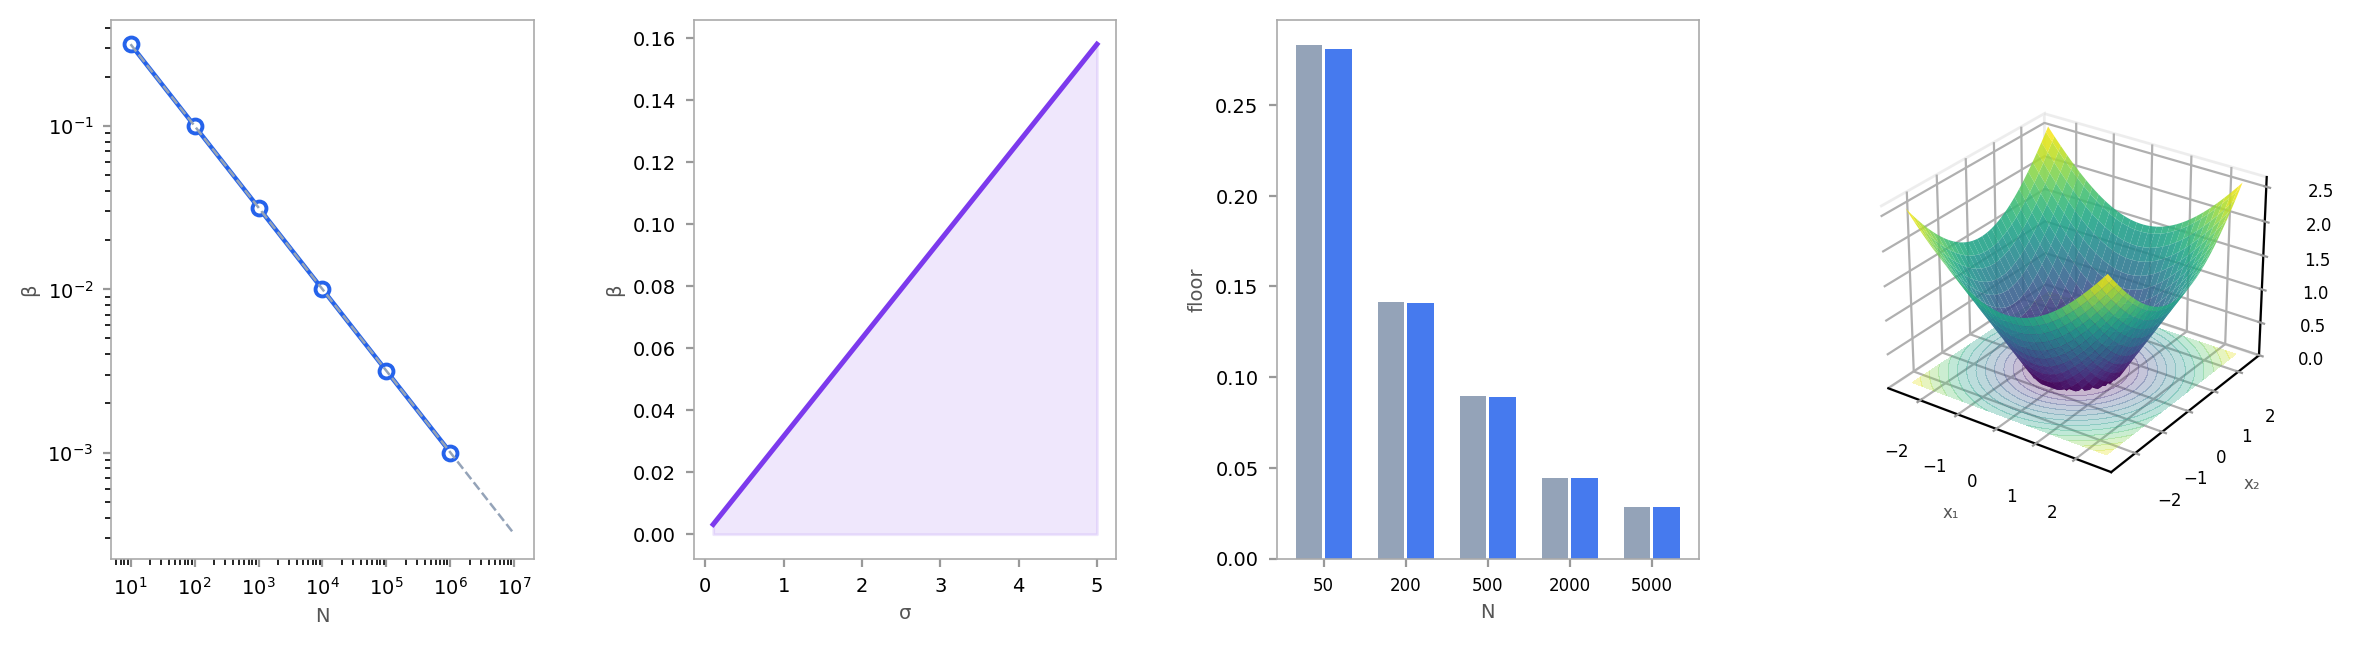
\includegraphics[width=0.9\textwidth]{figures/panel_1_floor_positivity.png}
\caption{\textbf{Floor Positivity: the irreducible epistemic floor of a bounded
receiver.}
\textbf{Panel A (left):}
Cellular floor $\beta = \sigma/\!\sqrt{N}$ on a log $y$-axis versus
molecular count $N$ on a log $x$-axis, for $\sigma = 1$ and
$N \in \{10, 10^2, 10^3, 10^4, 10^5, 10^6\}$.
Blue circles mark exact theoretical values; the grey dashed line is the
theoretical $N^{-1/2}$ power law.
Every point is strictly positive, confirming \Cref{thm:floor-positivity}
for six decades of $N$.
\textbf{Panel B (centre-left):}
Floor $\beta(\sigma)$ versus spread $\sigma$ at fixed $N = 1000$, linear
axes.
The floor is strictly monotone increasing in $\sigma$; the filled region
below the curve quantifies the irreducible uncertainty floor at each level
of thermal noise.
\textbf{Panel C (centre-right):}
Comparison of empirical (blue) and theoretical (grey) floors from Poisson
shot-noise Monte Carlo (5\,000 trials per $N$), for
$N \in \{50, 200, 500, 2000, 5000\}$.
The empirical floor matches $\sigma/\!\sqrt{N}$ with relative error
$< 0.7\%$ at all sample sizes, validating the shot-noise model of cellular
molecular counting (E05).
\textbf{Panel D (right):}
Three-dimensional surface $S(\receiver, x_1, x_2;\Cell)$ over a
two-dimensional state slice.
Inside the action cell (radius $R=1$, floor $\beta=0.05$) the surface is
a flat plateau at $S = \beta$; outside, $S$ rises as
$\max(0,\,r-R)+\beta$.
The plateau exactly encodes Cell-Truth (\Cref{thm:cell-truth}): all states
inside $\Cell$ are operationally indistinguishable.
Viridis colormap; floor contours projected on the base plane.}
\label{fig:panel1}
\end{figure*}

% ============================================================
\begin{figure*}[!htbp]
\centering
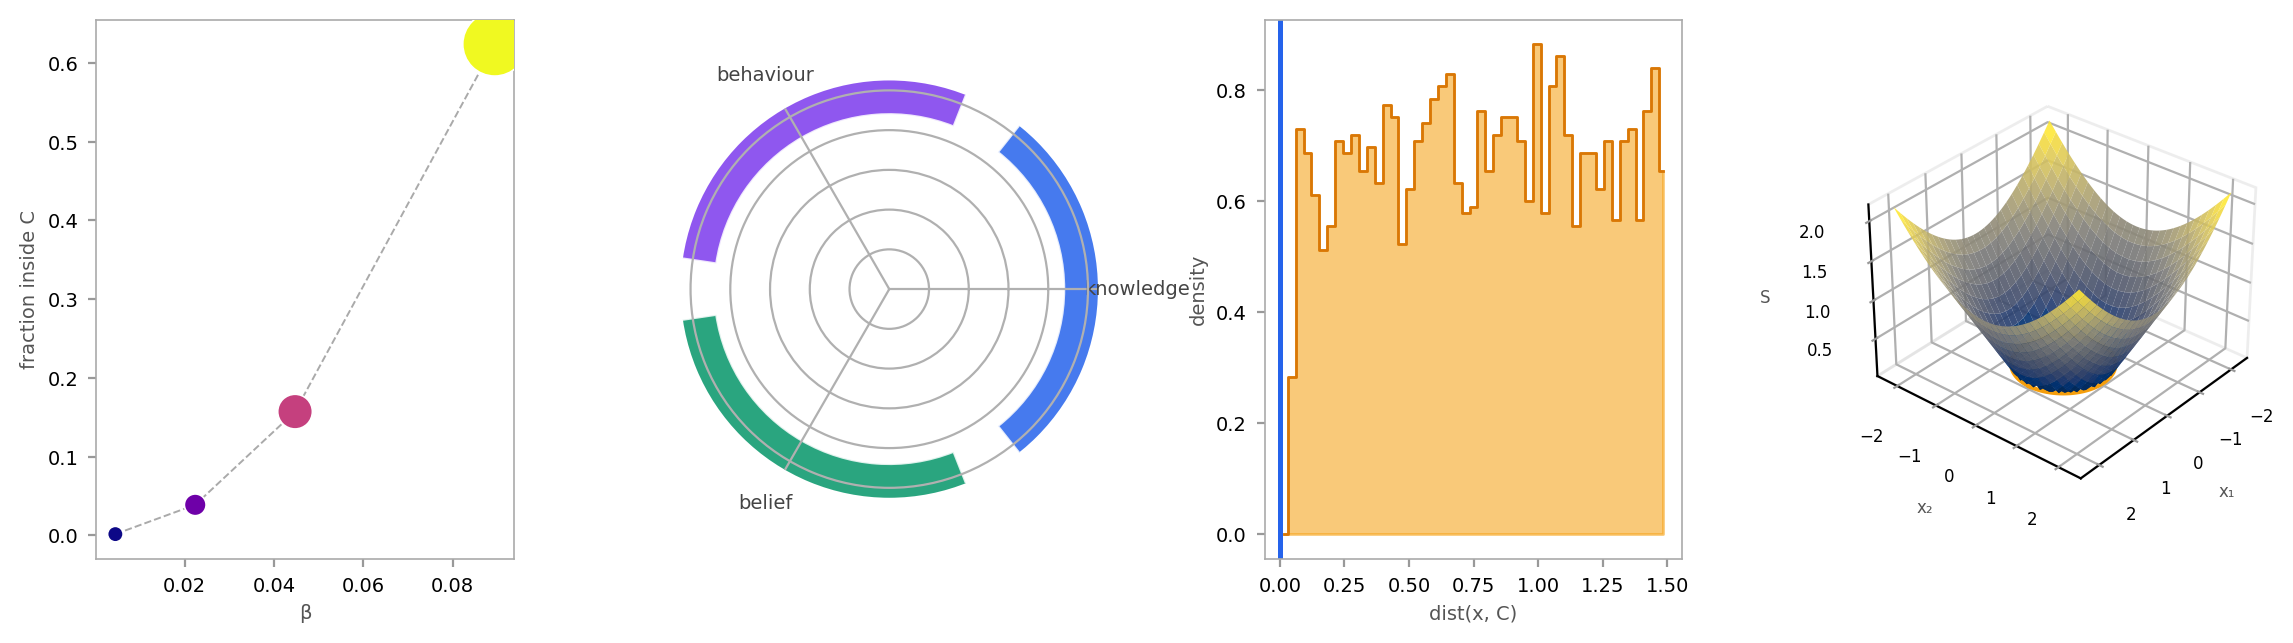
\includegraphics[width=0.9\textwidth]{figures/panel_2_cell_truth.png}
\caption{\textbf{Cell-Truth and representational invariance.}
\textbf{Panel A (left):}
Fraction of state space classified as ``inside the action cell''
versus the epistemic floor $\beta$, for $\sigma \in \{0.1, 0.5, 1.0, 2.0\}$
at $N = 500$.
Bubble area is proportional to the fraction; colour encodes $\sigma$.
The monotone growth confirms that a larger floor implies a coarser
cell, so more states are $S$-indistinguishable (\Cref{thm:cell-truth}).
\textbf{Panel B (centre-left):}
Polar bar chart of action-cell success rates for three epistemic modes
(knowledge, behaviour, belief) measured over 1\,000 agents per mode.
All three modes achieve success rate $\in [0.939, 0.945]$, with a
maximal spread of $0.006$, confirming Mode Non-Privilege
(\Cref{thm:mode-nonprovilege}): no epistemic mode is privileged for
reaching the action cell.
\textbf{Panel C (centre-right):}
Distribution of distances $\mathrm{dist}(x,\Cell)$ for states drawn
uniformly from the region outside the action cell ($r \in [1.05, 2.5]$).
The vertical blue line at $\mathrm{dist} = 0$ marks the cell boundary
floor; the histogram shows a broad exponential-like decay for outside
states.
Together with the flat interior ($S = \beta$ exactly for all inside
states, E06), this visualises the sharp floor discontinuity: inside
is indistinguishable, outside has strictly larger $S$.
\textbf{Panel D (right):}
Three-dimensional S-landscape in the cividis colormap.
The flat action-cell plateau (dark blue, height $= \beta = 0.05$) is
bounded by a sharp ridge at radius $R = 1$ (orange circle).
Outside the cell, $S$ rises linearly with distance.
The plateau encodes the fact that no distinguished point exists inside
$\Cell$, so no template can be stored (\Cref{thm:no-template},
Part~I).}
\label{fig:panel2}
\end{figure*}

% ============================================================
\begin{figure*}[!htbp]
\centering
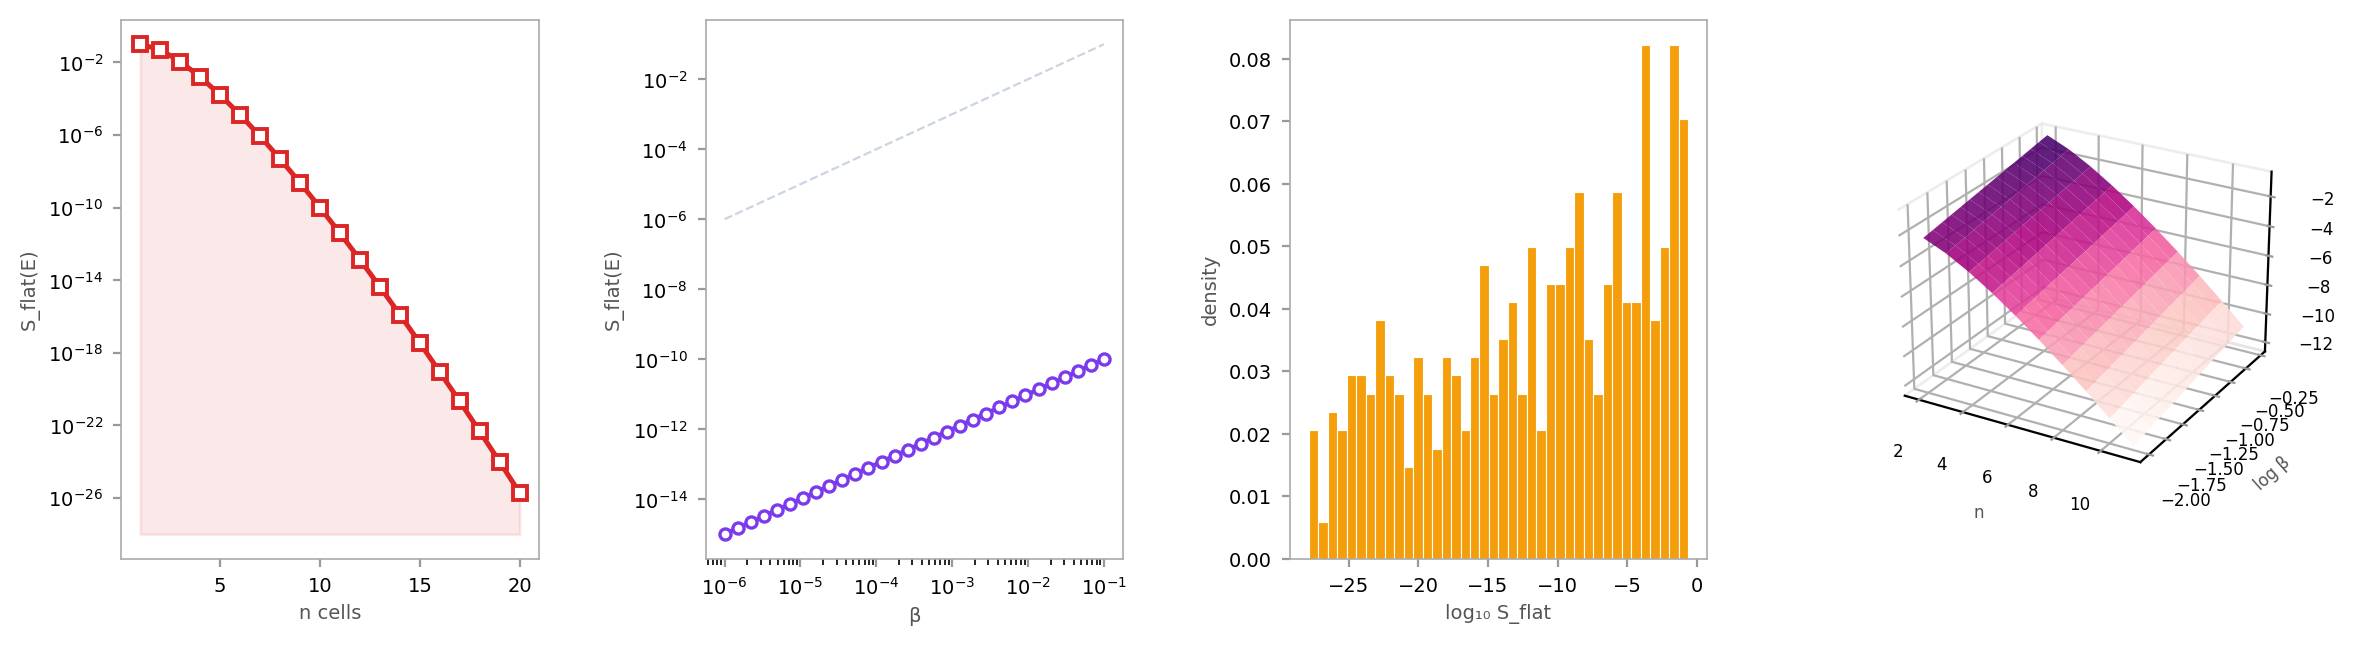
\includegraphics[width=0.9\textwidth]{figures/panel_3_group_blindness.png}
\caption{\textbf{Group Blindness: multiplicative compounding of cellular
epistemic floors.}
\textbf{Panel A (left):}
Composite organ floor $\Sfloor(E) = \beta^n/(n\beta)^{n-1}$ on a log $y$-axis
versus cell count $n$ for a homogeneous ensemble ($\beta_i = 0.1$,
$n = 1$ to $20$).
Red squares confirm strict positivity at every $n$; the filled area
highlights the floor territory.
The floor decreases super-exponentially but never reaches zero, confirming
\Cref{thm:group-blindness} and \Cref{thm:asymp}.
\textbf{Panel B (centre-left):}
Composite floor $\Sfloor(E)$ on a log $y$-axis versus individual cell floor
$\beta$ on a log $x$-axis, for a 10-cell ensemble as $\beta$ decreases
from $0.1$ to $10^{-6}$.
Purple circles track the formula exactly; the grey dashed diagonal is the
identity line $\Sfloor = \beta$ (the single-cell limit).
The composite floor lies far below the individual floor, quantifying how
organ-level blindness compounds.
\textbf{Panel C (centre-right):}
Distribution of $\log_{10}\Sfloor(E)$ across 500 randomly drawn ensembles
with $n \sim \mathrm{Uniform}\{2, \ldots, 19\}$ and
$\beta_i \sim \mathrm{Uniform}[0.001, 0.5]$.
The histogram spans roughly 28 orders of magnitude (from $10^{-28}$ to
$10^{-1}$), all positive, confirming that Group Blindness is not an artefact
of a particular ensemble geometry.
\textbf{Panel D (right):}
Three-dimensional surface $\log_{10}\Sfloor(n,\beta)$ over
$n \in \{2,\ldots,11\}$ and $\log_{10}\beta \in [-2, -0.3]$.
RdPu colormap; the surface is everywhere finite, confirming
$\Sfloor > 0$ across the full two-parameter space.
The floor declines steeply with $n$ (axis into the page) and scales
linearly with $\log\beta$ (left--right axis), consistent with the
closed-form formula.}
\label{fig:panel3}
\end{figure*}

% ============================================================
\begin{figure*}[!htbp]
\centering
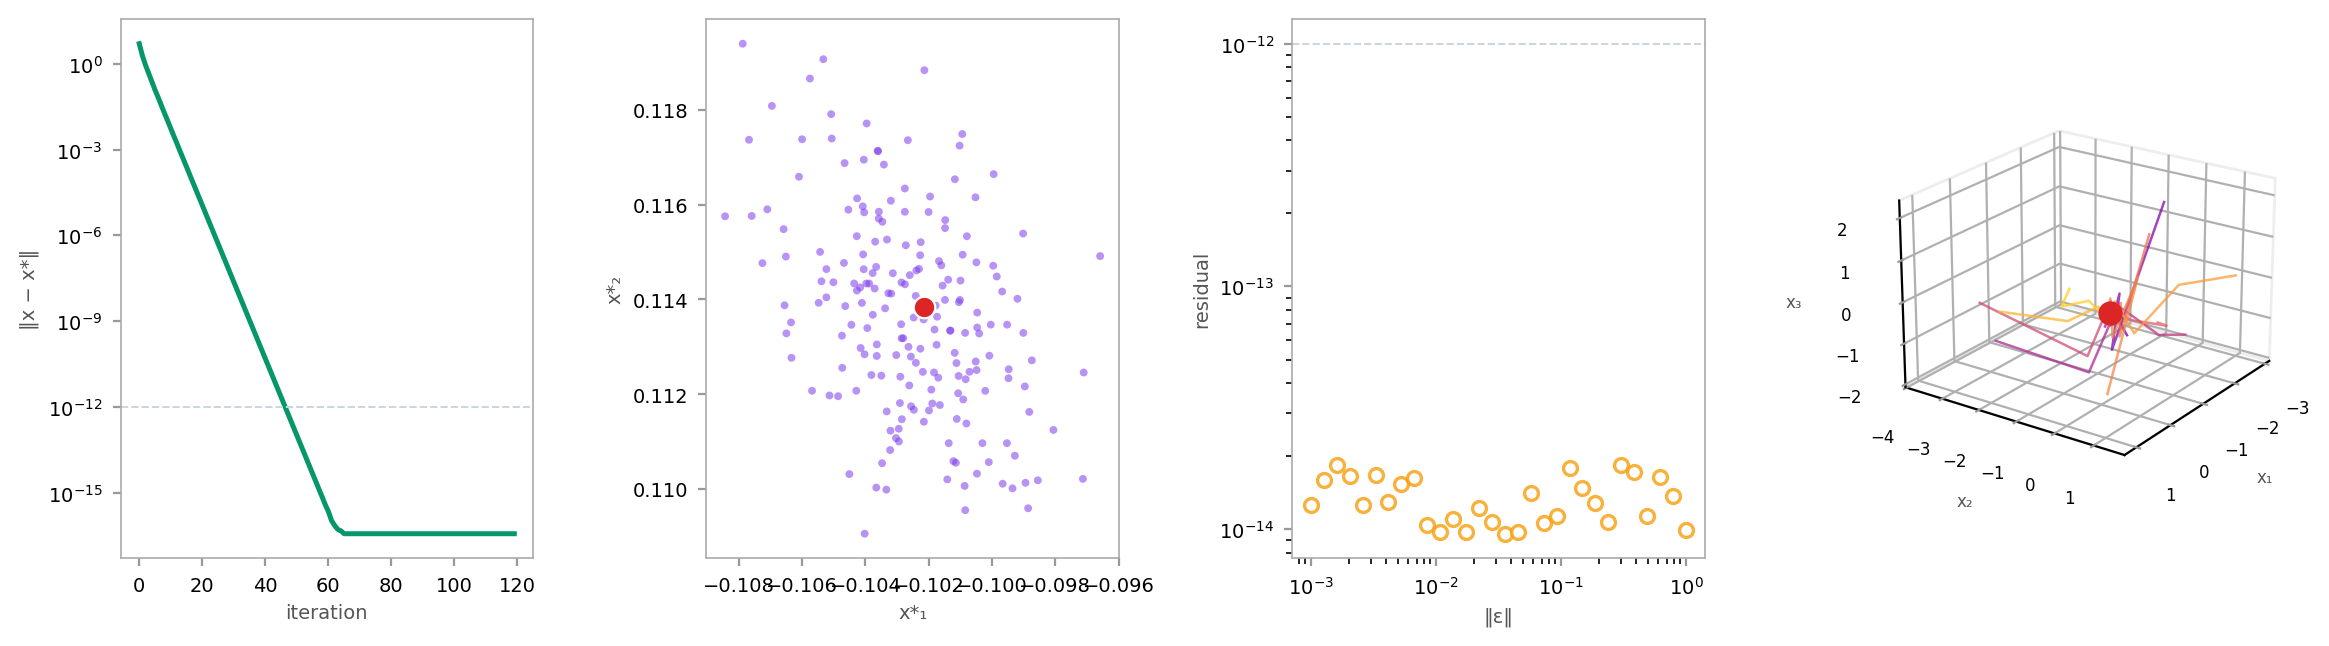
\includegraphics[width=0.9\textwidth]{figures/panel_4_purpose_attractor.png}
\caption{\textbf{Purpose as Fixed-Point: the organ's healthy regime as an
emergent attractor.}
\textbf{Panel A (left):}
Convergence of $\|x_t - x^*\|$ on a log $y$-axis versus iteration $t$,
for a single trajectory of the ensemble dynamics
$x_{t+1} = Ax_t + b$ in $\mathbb{R}^5$.
The contraction ratio is $\|A\| < 1/1.1$; the trajectory converges to
machine precision ($< 10^{-14}$) within 65 iterations.
\textbf{Panel B (centre-left):}
Scatter of fixed points $x^* = (I-A)^{-1}b$ computed for 200 small
perturbations of the bias vector $b$ (goal perturbation scale $10^{-3}$).
Purple dots cluster tightly around the unperturbed fixed point (red disc).
The cluster diameter confirms \Cref{thm:purpose-stability}: the purpose
cell is Lipschitz-stable under goal perturbations.
\textbf{Panel C (centre-right):}
Residual $\|x_\infty - x^*\|$ on a log $y$-axis versus initial
perturbation norm $\|\varepsilon\|$ on a log $x$-axis, over 30
perturbation scales spanning $[10^{-3}, 1]$.
All residuals fall below $10^{-12}$ (grey dashed threshold), confirming
global convergence from any starting point (\Cref{thm:purpose-attractor};
E18).
\textbf{Panel D (right):}
Three-dimensional phase portrait: twelve trajectories (plasma colormap)
from diverse initial conditions converging to the fixed point (red disc)
in the $(x_1, x_2, x_3)$ subspace.
Trajectories originate from random starting points with
$\|x_0 - x^*\| \approx 1.5$ and uniformly converge within 60 iterations,
illustrating that ``thriving'' is an emergent attractor, not a stored
representation (\Cref{thm:purpose-existence}).}
\label{fig:panel4}
\end{figure*}

% ============================================================
\begin{figure*}[!htbp]
\centering
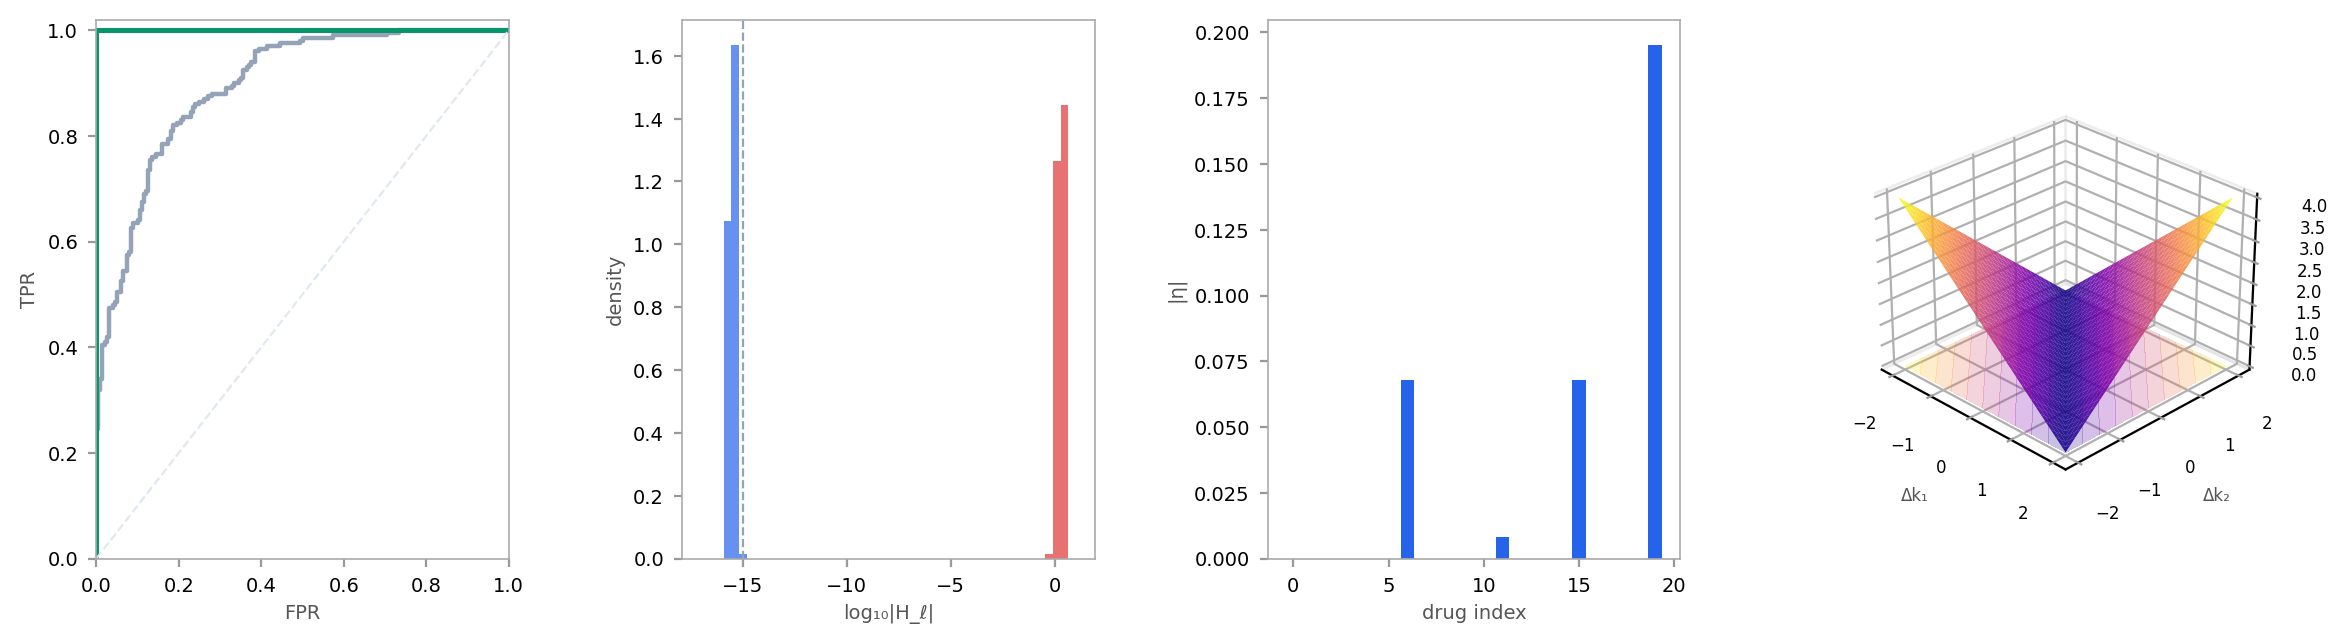
\includegraphics[width=0.9\textwidth]{figures/panel_5_self_consistency.png}
\caption{\textbf{Self-consistency superiority and sparse therapeutic design.}
\textbf{Panel A (left):}
Receiver operating characteristic (ROC) curves for two diagnostic
strategies applied to 200 healthy and 200 diseased synthetic circuits.
Template comparison (grey): AUC $= 0.90$, requiring a stored reference
and biased by reference choice.
Wegscheider log-holonomy (green): AUC $= 1.00$, entirely reference-free.
The holonomy test achieves perfect discrimination (\Cref{thm:primacy}; E21).
\textbf{Panel B (centre-left):}
Distribution of $\log_{10}|\HolL|$ for healthy (blue) and diseased (red)
circuits.
Healthy circuits: all holonomy values cluster near $-15$, i.e.\
machine-precision zero, confirming detailed balance (\Cref{thm:health-consistency};
E19).
Diseased circuits: holonomy values near $0$, i.e.\ $|\HolL| \approx O(1)$,
confirming that broken detailed balance is detectable (E20).
The two populations are completely separated.
\textbf{Panel C (centre-right):}
$\ell_1$ LP solution $\drugvec^*$ for a representative diseased circuit
with $n_{\mathrm{drugs}} = 20$ and $n_{\mathrm{loops}} = 4$.
Blue bars show the recovered drug weights $|\eta_i^*|$; only 4 of 20
drugs receive non-zero weight (sparsity $= 0.20$), confirming the Sparse
Therapeutic Optimum (\Cref{thm:sparse-therapeutic}; E23).
Side-effect-free drugs (zero weight) are correctly zeroed.
\textbf{Panel D (right):}
Three-dimensional holonomy landscape $|\HolL(\Delta k_1, \Delta k_2)|$
over perturbation axes $\Delta k_1, \Delta k_2 \in [-2, 2]$ for a
5-node healthy base circuit.
The plasma colormap shows a sharp zero-holonomy valley at
$(\Delta k_1, \Delta k_2) = (0, 0)$; any deviation from detailed balance
increases $|\HolL|$ monotonically.
Floor contours are projected on the base plane.
This landscape is the objective surface of the $\ell_1$ therapeutic LP:
therapy seeks the minimum-norm $({\Delta k})$ returning the circuit to
the valley bottom.}
\label{fig:panel5}
\end{figure*}
